\pagebreak
\subsection{Mechanical Design} \label{Mechanical_Design}


\subsubsection{Structure}

The experiment consists on two cubic boxes, one stacked over the other. The bottom box allocates the heaviest element, the CAC, as well as the Electronic Box (EB). The top box contains the AAC system. The frame of these two boxes will be made of aluminum bars which have a characteristic cross-section of 20x20 mm, see Figure \ref{cross-section}. The rails will allow an easy interface between bars and other elements. Bars with be joined together by using 90-degree angles, see Figure \ref{3_bars_joined}.

%% Cross section of one aluminum bar

\begin{figure}[!ht]
    \centering
    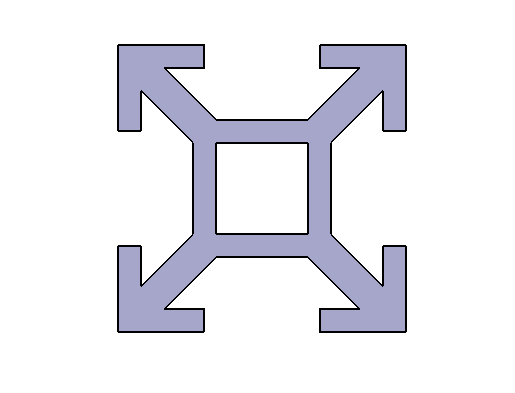
\includegraphics[width=0.5\textwidth]{4-experiment-design/img/1_cross_section.jpg}
    \caption{Cross section of the structural bars.}
    \label{cross-section}
\end{figure}

% Figure of 3 bars

\begin{figure}[!ht]
    \centering
    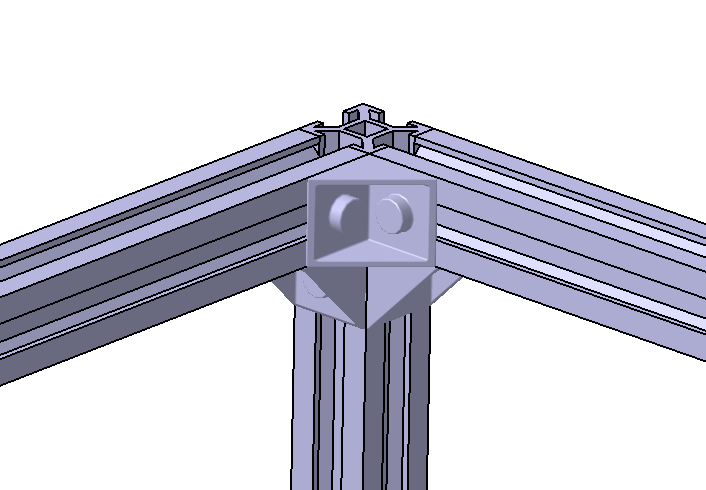
\includegraphics[width=0.6\textwidth]{4-experiment-design/img/bars_joint.jpg}
    \caption{Interface between structural bars.}
    \label{3_bars_joined}
\end{figure}

The design frame will be designed to withstand all vibrations and ensure a reliable stability of the entire system. 

The two-box design will allow ease of access and manipulation of both the CAC and AAC subsystems, see Figure \ref{strucutre}. In addition, the AAC sampling system is designed to be re-usable for future handover to FMI, as such, it will be mountable on any standard balloon flight without having to introduce major design changes.

% Figure of the two structures one above the other one (slightly separated)
\begin{figure}[!ht]
    \centering
    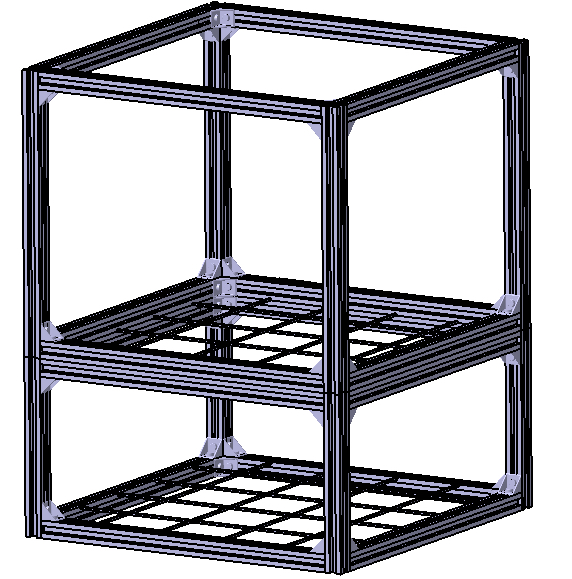
\includegraphics[width=0.7\textwidth]{4-experiment-design/img/frame_structure.jpg}
    \caption{Structure of the two-box design.}
    \label{strucutre}
\end{figure}

\subsubsection{CAC Subsystem}

The CAC Subsystem is designed around a the 300-meter coiled tube and the valve governing it. It will be placed at the bottom of the experiment box providing a stable location of the CoG. The coil will have a direct outside inlet and outlet by means of an extension tube reaching further from the gondola’s limits.

\pagebreak
\subsubsection{Electronics Box}

The OBC and its external elements will be allocated in the bottom of the experiment box taking advantage of the free space inside the doughnut shaped CAC coiled tube, see Figure \ref{electronics_box}. This location will help to protect it from the hazard outside environment. In addition, the heater will allow to regulate the temperature of this essential component.

%% Figure of the electronics box inside the coil, only bottom cube, isometric top view, explosion

\begin{figure}[!ht]
    \centering
    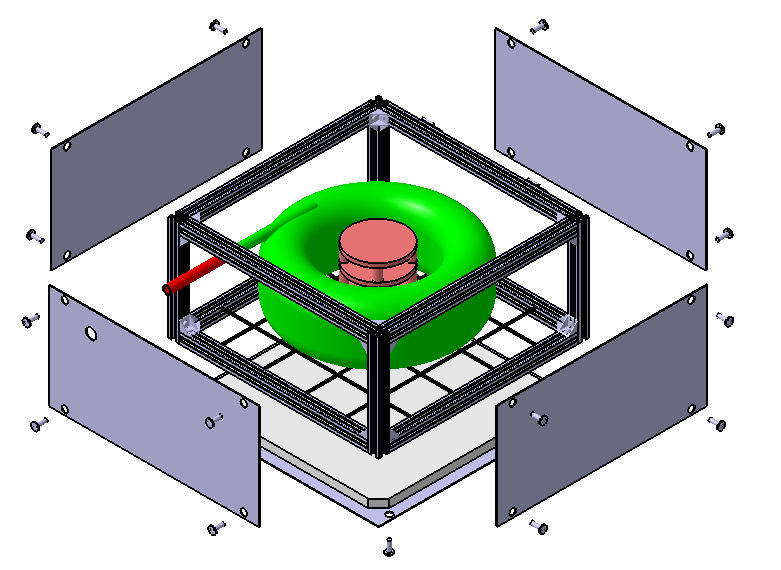
\includegraphics[width=0.7\textwidth]{4-experiment-design/img/explos_CAC.jpg}
    \caption{.}
    \label{electronics_box}
\end{figure}

\pagebreak
\subsubsection{AAC Subsystem}

The AAC Subsystem consists of 16 three liter sampling bags. Each bag will have a dedicated valve in the valve center to allow emptying and filling processes as well as to close the bag when needed. The bags will be placed vertically and will have two anchor points: on the top through a  multiple anchor interface (see Figure \ref{anchor_bags}) and on the bottom by means of the tubes connecting them to the valves.

%% Figure of the top box with its inside elements

\begin{figure}[!ht]
    \centering
    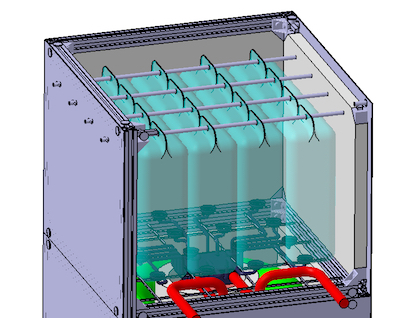
\includegraphics[width=0.7\textwidth]{4-experiment-design/img/anchored_bags.jpg}
    \caption{AAC Subsystem with all its elements.}
    \label{anchor_bags}
\end{figure}


\pagebreak
\subsubsection{Valve Center}

The valve center consists of a coated box to which the AAC's 16 air sampling bags will be attached to. This box will serve as the air flow chamber. It will be connected to a pipe from which outside air will be pumped and also enable pre-sample collection flushing, see Figure \ref{valve_center_and_pipes}. The pump providing the airflow will be allocated on the inlet side and protected by an air filter. 

%% Figure of the valve center with the pipe and small tubes

\begin{figure}[!ht]
    \centering
    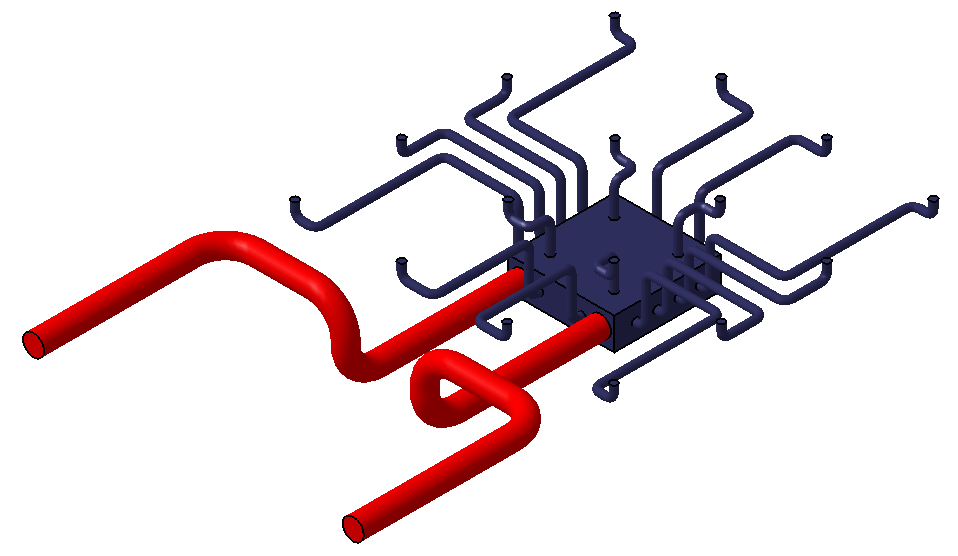
\includegraphics[width=0.9\textwidth]{4-experiment-design/img/valve_collector.jpg}
    \caption{Valve center with all the tubes to the sampling bags and to the outside environment.}
    \label{valve_center_and_pipes}
\end{figure}

\pagebreak
\subsubsection{Protection}

In order to protect the components from all kind of external elements, the experiment box will be shielded with removable aluminum walls along with a thick layer of Styrofoam attached to each wall. No internal space will be lost since the Styrofoam thickness is the same as that of the structural bars. Isolating sheets will also be glued in the walls to reinforce the temperature shielding. Each box has an internal aluminum mesh at the bottom face. It will help to protect the CAC coiled tube from impacts as well as to withstand its considerable mass. On the other hand, the mesh in the upper box is used to fix the valve center at a privileged centered position.

The walls will properly protect both the CAC coiled tube and the AAC sampling bags from any external element, unexpected rapid movements, and a probable hard landing impact. Cross-section in Figure \ref{cut_all}. 


%% Cut: Figure CAC+EB, AAC+valve center, and walls + Styrofoam.

\begin{figure}[!ht]
    \centering
    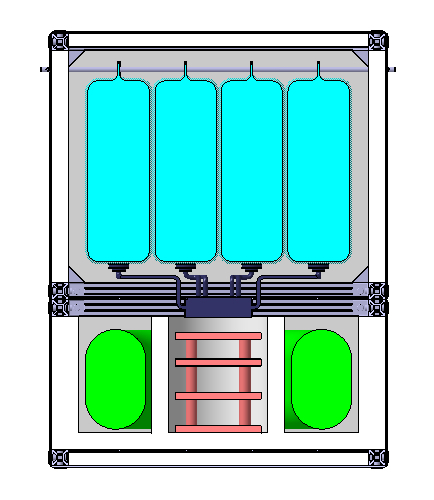
\includegraphics[width=0.7\textwidth]{4-experiment-design/img/tall_frontal.jpg}
    \caption{Cross-section of the whole experiment box.}
    \label{cut_all}
\end{figure}

The front walls, face of the experiment box exposed to the outside, will have several holes to allow the tubes providing air flow to collect clean air from the outside, see Figure \ref{front_wall_holes}.

The top lateral walls will have four holes to allow the introduction of the circular bars used as anchor points for the sampling bags, see Figure \ref{anchor_bags}.

Bolts shall be used to attach all walls to the structure's railed bars.

%% Figure front wall holes: isometric

\begin{figure}[!ht]
    \centering
    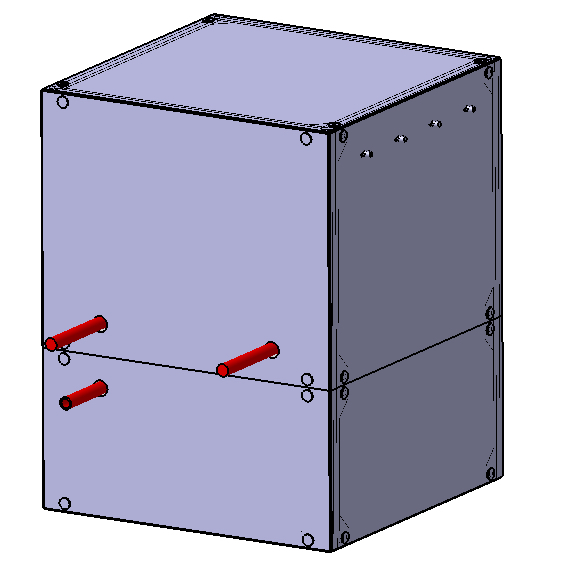
\includegraphics[width=0.7\textwidth]{4-experiment-design/img/frontal_holes.jpg}
    \caption{.}
    \label{front_wall_holes}
\end{figure}

\pagebreak
\subsubsection{Fixing Interface}

The two experiment box subsystem structures will be joined together by two mechanisms. On the front side, two flat plates with two bolts each will interface both structures. On the back side, two hinges will be used to allow a controlled rotation of the structure above, see Figure \ref{open_box_1}. This method will allow for easy and fast access to all the elements allocated inside the experiment box, see Figure \ref{open_box_2}. The latter implies a comfortable manipulation of both electrical and pipes connection between the EB and the valve center as well as each bags with its dedicated valve. 

Quick access to the CAC coiled tube is provided so that it may be quickly extracted for post-flight analysis.

%% Figure of experiment box open 1

\begin{figure}[!ht]
    \centering
    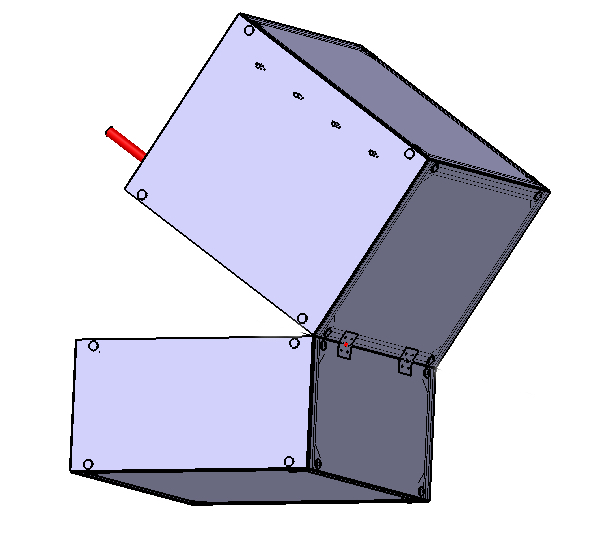
\includegraphics[width=0.7\textwidth]{4-experiment-design/img/hinges.jpg}
    \caption{Detail of hinges mechanism.}
    \label{open_box_1}
\end{figure}

%% Figure of experiment box open 2

\begin{figure}[!ht]
    \centering
    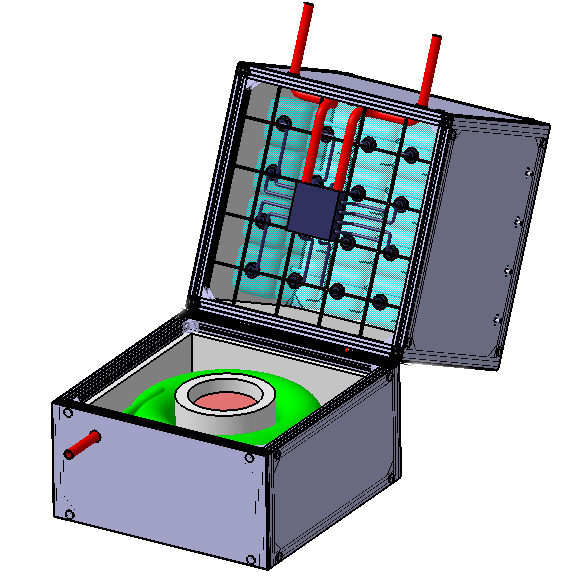
\includegraphics[width=0.7\textwidth]{4-experiment-design/img/open_box.jpg}
    \caption{View of the experiment box open for manipulation.}
    \label{open_box_2}
\end{figure}

\pagebreak
\subsubsection{Manipulation Interface}

The two-box system will be fixed to the gondola rails by using four 90-degree angles, 2 per rail. The low line CoG acts as a crucial characteristic for stability. Top anchors could be also used if requested. 


Several handles will be placed to allow an easy and safe manipulation of the experiment box. 


\subsubsection{Mechanical Components}

All the components used in the mechanical design can be found in Table \ref{tab:mechanical-components}. Spare elements are not included. 


\raggedbottom